\textit{Student's concept of writing}\label{chapter:research_results_students_findings}
\begin{table*}[b]
\centering
\caption{Students' Report Writing Following Writing Guidelines}
\begin{tabular}{|l|c|}
 \hline
    \textbf{Writing guidelines}&\textbf{Students following guidelines/Total number of students}\\
 \hline
    Global content (IMRD)&\\
 \hline 
    Organizational pattern (chapters)&\\
 \hline
   & \\
 \hline 
   & \\
 \hline
    &\\
 \hline
   & \\
 \hline
\end{tabular}
\label{table:frequent_writing_considerations}
\end{table*}
\textit{Teacher's concept of writing}
\label{chapter:research_results_teacher_findings}
\input{chapters/research/research_expertise/research_results/research_results_teacher_findings}
\textit{Limitations in teaching academic writing}
\label{chapter:research_results_limitations}
\input{chapters/research/research_expertise/research_results/research_results_limitations}
\textit{Improving teaching academic writing}
\label{chapter:research_results_improvements}
\input{chapters/research/research_expertise/research_results/research_results_improvements}


% \begin{table*}[t]
% \centering
% \caption{Pre-development and post-development of the \acrshort{ale} course material per student group with results of statistical analyses}
% \resizebox{\textwidth}{!}{%
% \begin{tabular}{p{3.5cm} p{3.5cm} p{3.5cm} p{3.5cm}}
%  \hline
%      & Cumulative ALE score 
%      %Mean $\%$ score ($\pm$ SD)
%      $N$ &  ANOVA test comparing group performance & Kruskal Wallis H test  comparing group performance \\
%     \hline
%     Control group  & 50 & $p>0.1$ & $p>0.1$ \\
%     (pre-development)&&&\\
%     Test group     &1 & - & -  \\ 
%     (post-development)&&&\\
% \hline
% $N$ number of students&&&\\
% \end{tabular}%
% }
% \label{table:statistical_analysis_scores_different_groups}
% \end{table*}

% \Cref{table:statistical_analysis_scores_different_groups}  and \Cref{table:statistical_analysis_scores_same_group} show the results of the statistical analyses tests performed in this study.
% First, a comparison between past \acrshort{ale} iteration was made to identify differences.
% \Cref{fig:distribution1820} shows the score distribution for pre-development course material student groups. 
% To satisfy the ANOVA independency condition, students which attended both \acrshort{ale}1 and \acrshort{ale}2 had their scores averaged, yielding to each group containing independent samples. 
% While data is normal, group 1920ss is positively skewed. 
% Assuming normality, with ANOVA the $p$-value is greater than 0.1. With Kruskal Wallis H-test the $p$-value also exceeds 0.1, thus, in conclusion, there is no statistical difference between the scores of previous \acrshort{ale} course iterations. The post-development group was also included and tested with ANOVA and Kruskal Wallis H. Similarly, student scores from group 22021fw were averaged to satisfy independency.\\\\
% %However, no significant difference was identified with the post-development comparison.\\\\
% %The paired t-test was conducted on the 22021fw which had both pre-development and post-development course material.[TODO]\\\\
% %\Cref{fig:distribution2021fw} shows the score distribution for the pre and post-development course material. [TODO]\\\\
% %This test yielded a $p<0.05$ which indicates that there is a significant difference between student performance with the new course material.
% %Looking at the distribution it is clear that 2021fw2 group performed better. \\\\
% Furthermore, there is not significant difference in the performance of past \acrshort{ale} student groups.
% \Cref{appendices:scores} describes a detailed study of the test group 1920ss for which the statistical analysis proved significant evidence in comparing \acrshort{ale}1 with \acrshort{ale}2 performance. For this group, although there seems to be a difference in performance, the performance in \acrshort{ale}2 is worse due to the introduction of weekly deadlines and mandatory feedback sessions. Moreover, having participated in the \acrshort{ale}1 course, the students should be familiar with the workload and requirements. However, while a few students score slightly better, majority seems to perform worse in \acrshort{ale}2. This may also be due to the fact that students usually join some electives to fill in missing \Gls{ec}s and deliver up to a passing grade. Thus, further research is required to assess student performance in both \acrshort{ALE} courses. Also, the study should be performed on larger groups, as the current test group was too formed of too little students.\\\\
% Unfortunately, the second part of the course had one student left for assessment. While several students joined in the beginning, majority dropped till the end, yielding a test group formed of 1 student that has followed both \acrshort{ale}1 and \acrshort{ale}2. Hence, the statistical testing could not be performed anymore for this test group.


% \begin{table*}[t]
% \centering
% \caption{\acrshort{ale} scores per student group with results of statistical analyses}
% \resizebox{\textwidth}{!}{%
% \begin{tabular}{p{3.5cm} p{3.5cm} p{3.5cm} p{3.5cm}}
%  \hline
%      & Cumulative ALE score Mean $\%$ score ($\pm$ SD) $N$ &  Paired t-test comparing ALE1 with ALE2 performance &  Wilcoxon signed-rank test comparing ALE1 with ALE2 performance\\
%  \hline
%     1718ss & $7.97\pm1.26$ & $p>0.1$ &\\
%     &5&&\\
%     1819fw & $8.78\pm0.78$& &  $p>0.1$\\
%     &8&&\\
%     1819ss & $8.33\pm0.69$& $p>0.1$ &\\
%     &8&&\\
%     1920fw & $8.25\pm1.25$& - &  -\\
%     &1&&\\
%     1920ss & $7.3\pm1.22$& & $p<0.05$\\
%     &10&&\\
%     2021fw & & -& -\\
%     &1&&\\
%      \hline
% SD standard deviation, & $N$ number of students&&\\
% \end{tabular}%
% }
% \label{table:statistical_analysis_scores_same_group}
% \end{table*}


% \begin{figure}[h]
%     \centering
%     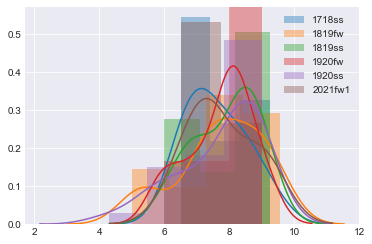
\includegraphics[width=0.7\textwidth]{figures/distribution.png}
%     \caption{\acrshort{ale} integral assessment scores distribution for the 2018-2020 student groups}
%     \label{fig:distribution1820}
% \end{figure}
% % \begin{figure}[h]
% %     \centering
% %     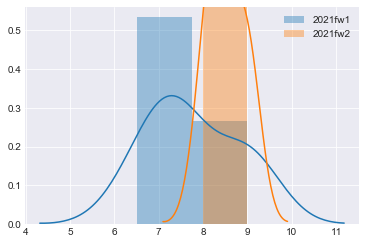
\includegraphics[width=0.7\textwidth]{figures/distribution2021fw-mock.png}
% %     \caption{\acrshort{ale} integral assessment scores distribution for the 2020-2021 Fall/Winter semester student group}
% %     \label{fig:distribution2021fw}
% % \end{figure}